\chapter{Конструкторская часть}

В этой части будут представлены требования к программному обеспечению, описание структур данных и схемы выбранных алгоритмов.

\section{Описание структур данных}

В разрабатываемом программном обеспечении будут использоваться следующие структуры данных:
\begin{enumerate}[label=\arabic*)]
	\item сцена состоит из списка объектов и списка источников света;
	\item каждый объект сцены задается списком его вершин и полигонов;
	\item полигон включает в себя индексы 3 точек, цвет и оптические свойства поверхности, которую задает этот полигон;
	\item цвет состоит из 4 чисел;
	\item источник света определяется 3 координатами, которые задают положение в пространстве, и интенсивностью света.
\end{enumerate}

\section[Общий алгоритм визуализации трехмерной сцены]{Общий алгоритм визуализации\\трехмерной сцены}

Общий алгоритм визуализации сцены:
\begin{enumerate}[label=\arabic*)]
	\item загрузка и обработка файлов с объектами сцены (фламинго);
	\item задание расположения фламинго и источников света;
	\item генерация растительности, учитывая плотность;
	\item получение видимых граней и поверхностей, используя алгоритм z-буфера;
	\item нахождение отражений растительности и фламинго относительно озера;
	\item получение теней, используя модифицированный алгоритм z-буфера;
	\item отрисовка изображения.
\end{enumerate}

Формализованная модель разрабатываемого программного обеспечения в виде IDEF0 диаграммы 1 уровня изображена на рисунке~\ref{fig:idef1}.

\begin{figure}[h!]
	\centering
	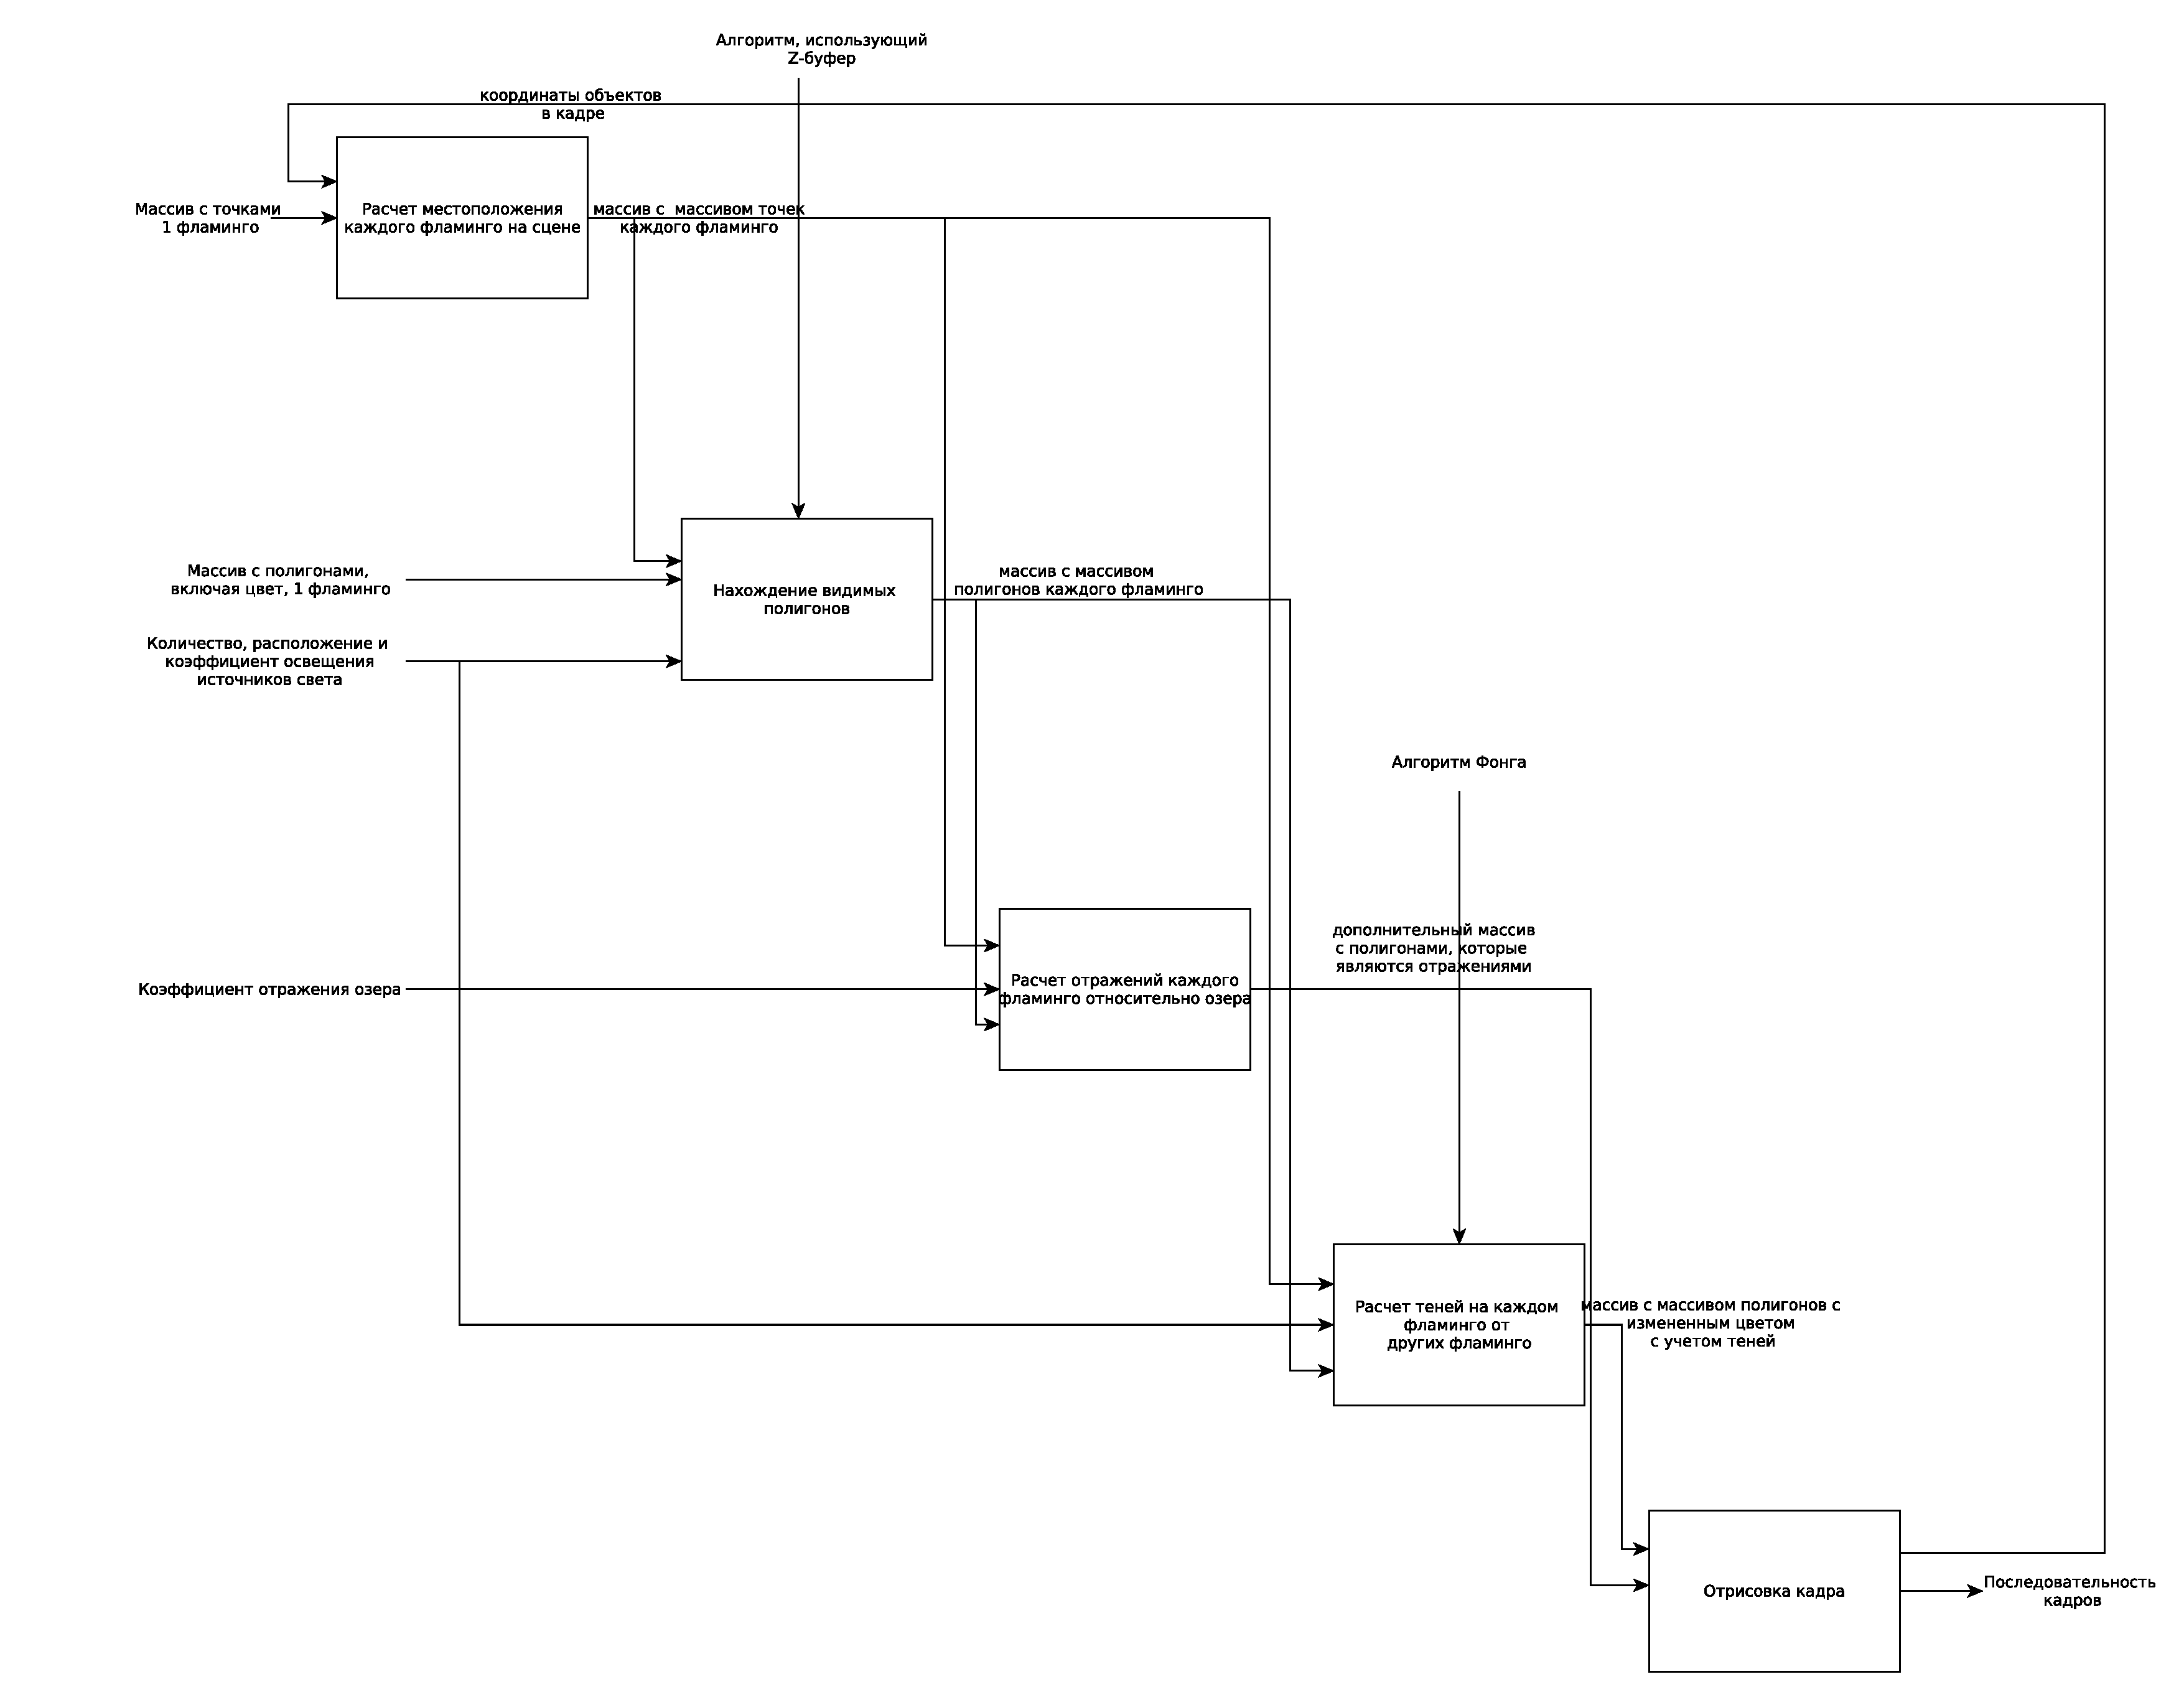
\includegraphics[width=\linewidth]{img/idef1}
	\caption{IDEF0 диаграмма, 1 уровень}
	\label{fig:idef1}
\end{figure}


\section{Алгоритм, использующий z-буффер}

Схема алгоритма представлена на рисунке~\ref{fig:z}.

\begin{figure}[h!]
	\centering
	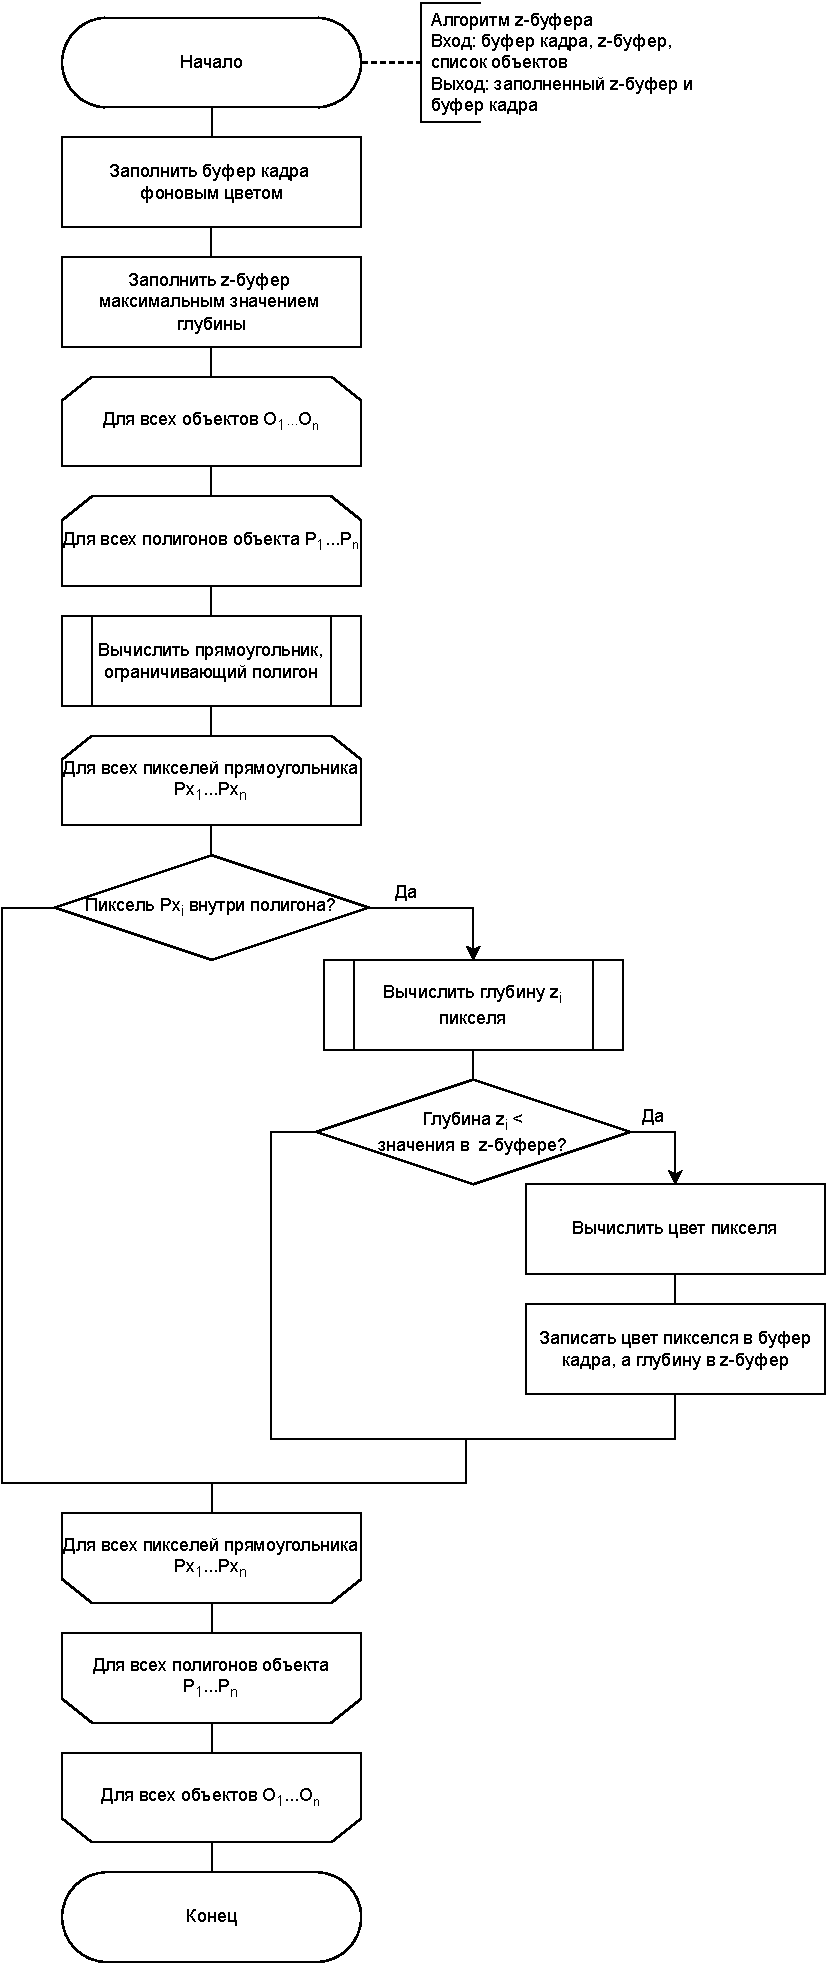
\includegraphics[width=0.65\linewidth]{img/z}
	\caption{Схема алгоритма, использующего z-буфер}
	\label{fig:z}
\end{figure}
\clearpage

\section[Модификация алгоритма, использующего z-буффер, для нахождения теней]{Модификация алгоритма,\\использующего z-буффер, для\\нахождения теней}

Схема модицифицированного алгоритма, использующего z-буффер, для нахождения теней представлена на рисунке~\ref{fig:z_mod}.

\begin{figure}[h!]
	\centering
	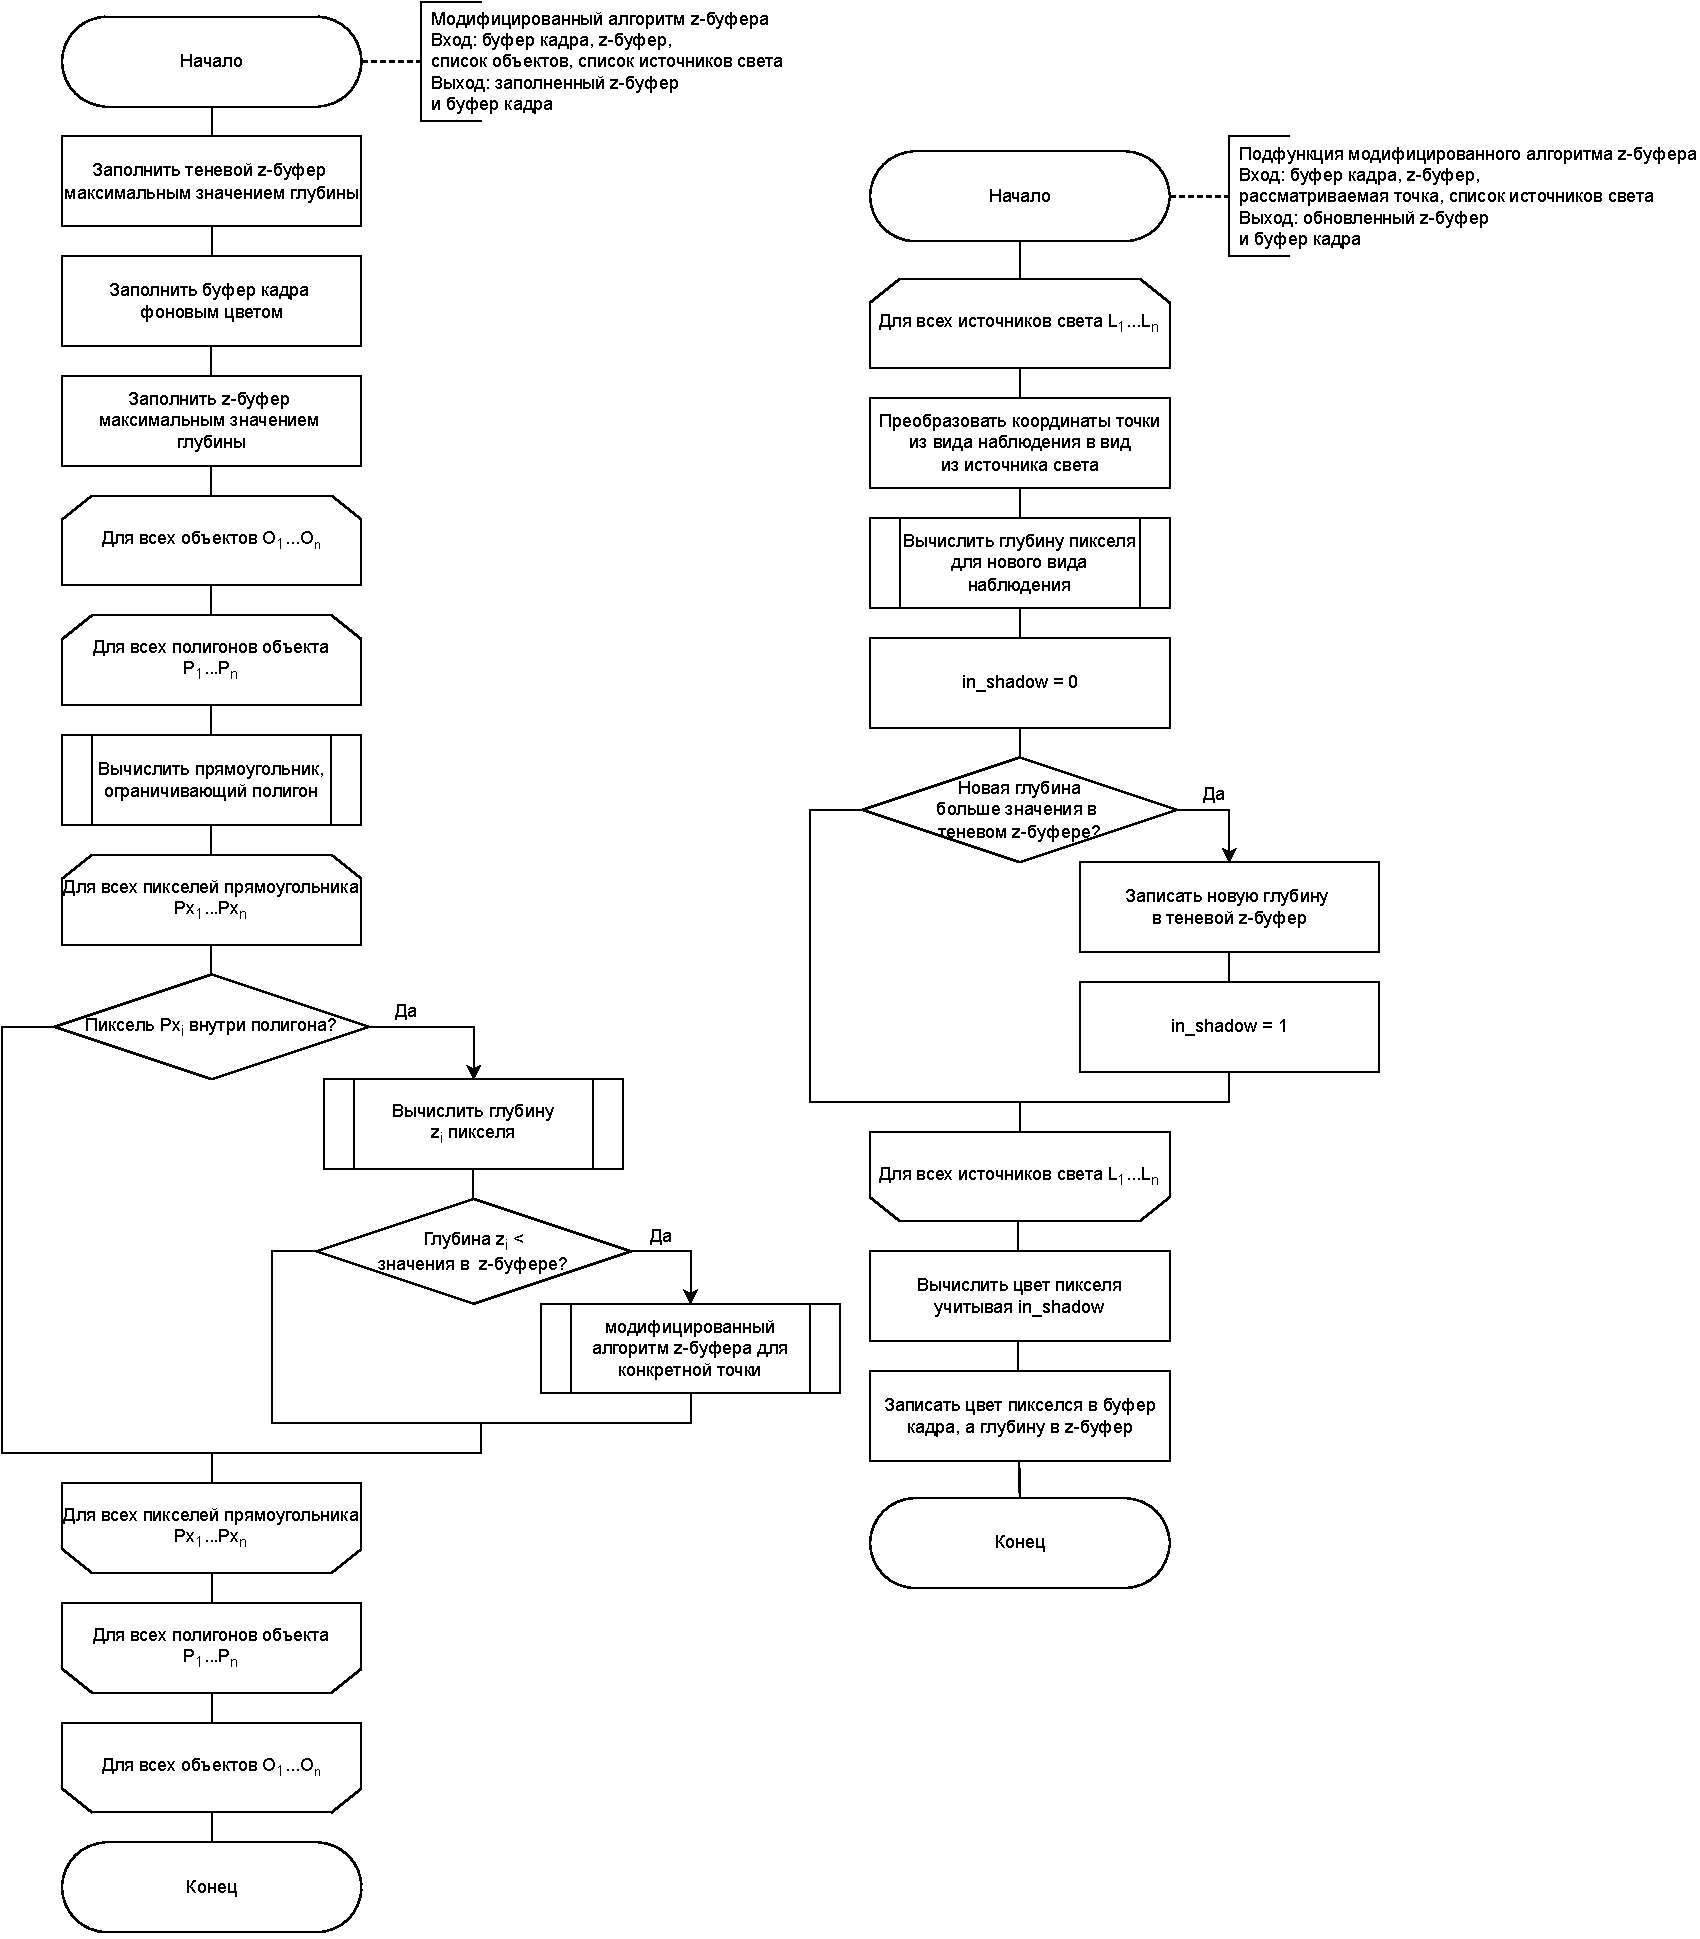
\includegraphics[width=0.96\linewidth]{img/z_mod}
	\caption{Схема модифицированного алгоритма, использующего z-буфер}
	\label{fig:z_mod}
\end{figure}
\clearpage

\section{Алгоритм для отображения отражений}

Точка $P$ и ее отраженная относительно плоскости отражения точка $P'$ связаны следующим выражением: 
\begin{equation}
	\label{for:ref}
	P' = P - 2\frac{N \cdot P}{\|N\|^2} \cdot N,
\end{equation}
где $N$ - вектор нормали к плоскости отражения~\cite{refl}.

Схема алгоритма для расчета отражений представлена на рисунке~\ref{fig:reflect}.

\begin{figure}[h!]
	\centering
	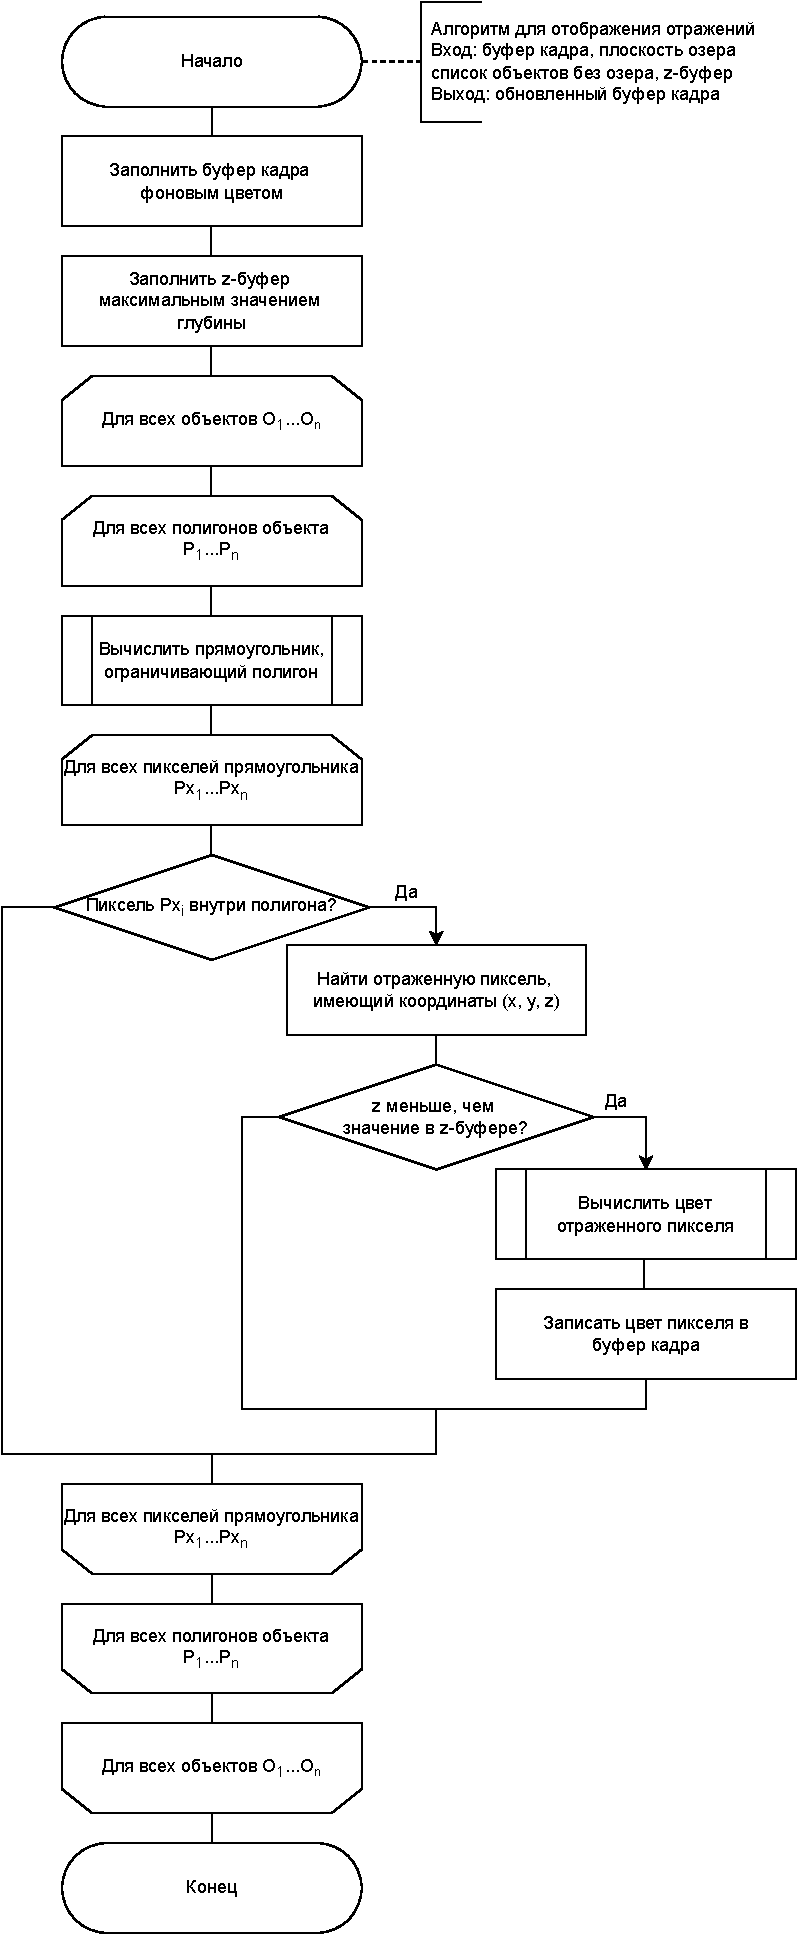
\includegraphics[width=0.62\linewidth]{img/reflect}
	\caption{Схема алгоритма для отображения отражений}
	\label{fig:reflect}
\end{figure}
\clearpage

%\section{Алгоритм для визуализации ходьбы фламинго}

%Для визуализации ходьбы фламинго нужно расчитать функцию движения его коленей и ступней.

\section*{Вывод}

Было спроектировано программное обеспечение для построения трехмерной сцены и визуализации озера с растительностью и фламинго.